\begin{frame}
\frametitle{Hardware used in this training session}
  BeagleBone Black, from CircuitCo
  \begin{columns}
    \column{0.6\textwidth}
    \footnotesize
    \begin{itemize}
      \item Texas Instruments AM335x (ARM Cortex-A8)
      \item Powerful CPU, with 3D acceleration, additional processors
        (PRUs) and lots of peripherals.
      \item 512 MB of RAM
      \item 2 GB of on-board eMMC storage
      \item USB host and USB device ports
      \item microSD slot
      \item HDMI port
      \item 2 x 46 pins headers, with access to many expansion busses
        (I2C, SPI, UART and more)
      \item A huge number of expansion boards, called {\em capes},
        available on the market
    \end{itemize}
    \column{0.4\textwidth}
    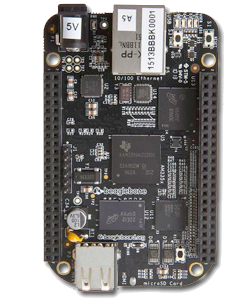
\includegraphics[width=\textwidth]{slides/kernel-beagleboneblack/beagleboneblack.png}
  \end{columns}
\end{frame}
